\documentclass[11pt, a4paper, twocolumn]{ieeeconf}
\raggedbottom

\usepackage{amsfonts}
\usepackage{blindtext}
\usepackage{geometry}
\usepackage{setspace}
% \usepackage{titlesec}
\usepackage{indentfirst}
\usepackage{graphicx}
\usepackage[italian]{babel}
\usepackage{catchfile} % used in \getenv command
\usepackage{multicol}
\usepackage{amsmath}
\usepackage{subcaption}
\usepackage[hang, flushmargin, multiple, bottom]{footmisc}
\usepackage{float}
\usepackage{array}
\usepackage{booktabs}
\usepackage{url}
\usepackage{csvsimple}
\usepackage{framed}

%\titlespacing*{\section}{0px}{3mm}{1mm}
%\titlespacing*{\subsection}{0px}{3mm}{1mm}
\geometry{
  left=2cm,
  right=2cm,
  top=2cm,
  bottom=2cm
}

\graphicspath{ {./assets}, {../../assets} }

% Allow use of command \getenv{VARNAME}.
% Taken from: https://tex.stackexchange.com/questions/62010/can-i-access-system-environment-variables-from-latex-for-instance-home
\newcommand{\getenv}[2][]{
  \CatchFileEdef{\temp}{"|kpsewhich --var-value #2"}{\endlinechar=-1}%
  \if\relax\detokenize{#1}\relax\temp\else\let#1\temp\fi}

% Roman numerals
\newcommand{\rom}[1]{\uppercase\expandafter{\romannumeral #1\relax}}

% authors, date and title---------------------------------------------------------------
\author{Matteo Bonacini \\ \getenv{MAT1}}
\date{\today}
\title{Controllo di un pendolo invertito su rotaia}
%---------------------------------------------------------------------------------------
\begin{document}

  \twocolumn[
    \begin{@twocolumnfalse}

      \maketitle
      \begin{abstract}\label{sec:abstract}
Abstract
\end{abstract}


    \end{@twocolumnfalse}
  ]

  \section{Introduzione}\label{sec:introduzione}
\subsection{Pendolo invertito}\label{subsec:intro-pendolo}
Il pendolo invertito su rotaia è un sistema che si presta molto bene ad essere trattato nell'ambito della Teoria del
Controllo.
Il problema che ci poniamo è il seguente:
\begin{framed}
\emph{
    Un pendolo è posto su un carrello libero di muoversi orizzontalmente su una rotaia.
    Il carrello è dotato di un motore che gli permette di accelerare. Conoscendo lo stato del sistema
    $\mathbf x$, trovare un espressione per la forzante esercitata dal motore $\mathbf u = \mathbf u(\mathbf x)$ che faccia sì
    che il pendolo rimanga orientato verso l'alto.
  }
\end{framed}

Una descrizione formale del sistema è data dal diagramma in fig. %todo add ref
% todo add figure
dove $\mathbf y$ è l'output del sistema, $\mathbf x$ e $\mathbf f$ sono rispettivamente
lo \emph{stato interno} e la \emph{legge di evoluzione} del sistema. $\mathbf y$, $\mathbf x$ e $\mathbf f$ sono
\emph{vettori colonna}.

Sebbene sia possibile risolvere questo problema per qualsiasi condizione iniziale del sistema, io tratterò solo il
caso in cui il pendolo parte già in prossimità della posizione verticale. Strategie di \emph{swing-up} e
\emph{swing-down} non saranno oggetto del mio studio.


\subsection{Controller \textsc{LQR}}\label{subsec:intro-lqr}
In generale, nello studio del controllo di un sistema, dobbiamo tenere in considerazione del fatto che la forzante
$\mathbf u$ ha un certo costo associato.
Questo è da intendersi sia come costo \emph{materiale} (i.e. il costo della corrente per mettere in moto
un motore) ma, soprattutto, anche come costo \emph{fisico} (i.e. non si può realizzare un motore che ha potenza
infinita).

Un controller \textsc{lqr}, permette di risolvere questi vincoli in modo \emph{ottimale}. %todo ref
Per spiegare cosa si intende con \emph{ottimale}, conviene citare direttamente la definizione di \textsc{lqr}, seguita
da un teorema:
% also todo, magari cita il libro di Brunton

\begin{framed}
  \textbf{DEF}
  Un controller \textsc{lqr} è un sistema dinamico con input $\mathbf y$, output $\mathbf u$ e stato interno
  $\hat{\mathbf x}$: %fixme questa è la def di lqg
  \begin{equation}
    \begin{aligned}[c]
      \frac d {dt} \hat {\mathbf x} &= (A-K_f C - B K_r) \hat{\mathbf x} + K_f \mathbf y \\ %fixme matrices need to be not itlaics
      \mathbf u               &= -K_r \hat{\mathbf x}
    \end{aligned}
    \label{eq:lqr}
  \end{equation}
\end{framed}
\begin{framed}
  \textbf{THM}
  Il controller descritto in \eqref{eq:lqr} minimizza la funzione costo definita come:
  \begin{equation}
    J(t) \doteq
      \int_0^{+\infty} \left[ \mathbf{x} (s)^* Q \mathbf {x} (s) + \mathbf {u} (s)^* R \mathbf {u} (s) \right] ds
    \label{eq:lqr-costo}
  \end{equation}
\end{framed}

Non entrerò nel dettaglio riguardo a quali sono le condizioni per cui si può realizzare un controller di questo tipo.
Inoltre, ci tengo a precisare che sebbene le equazioni sopra %todo add ref)
valgano per sistemi dinamici a \emph{tempo continuo}, si possono generalizzare tranquillamente a sistemi
a \emph{tempo discreto}.
Rimando a Brunton%todo cite
per approfondimenti.

\subsection{Controller \textsc{PID}}\label{subsec:intro-pid}
%todo da fare

  \section{Modello e implementazione del sistema}\label{sec:modello}
\subsection{Modello del sistema}\label{subsec:modello-del-sistema}
Il sistema del pendolo invertito è riassunto in figura \ref{fig:sistema}.
In questa sezione ricaverò le equazioni del moto e le linearizzerò attorno al punto di equilibrio instabile.

\begin{figure}[h]
    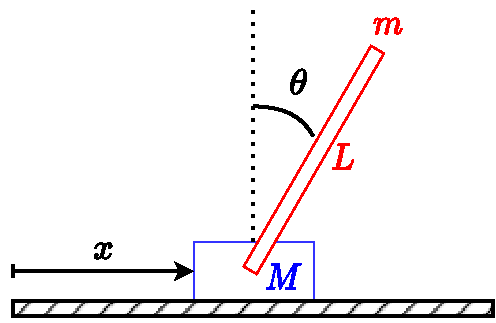
\includegraphics{../assets/sistema.pdf}
  \caption{\emph{Pendolo invertito. Le coordinate generalizzate sono $x$ e $\theta$. Il carrello ha massa $M$,
  il pendolo ha lunghezza $L$ e massa $m$. Un motore (non rappresentato in figura) esercita una forza che agisce
  lungo $\hat x$. Si noti che la coordinate generalizzata $x$ e lo stato del sistema $\bf x$ sono due grandezze diverse.}}
  \label{fig:sistema}
\end{figure}


La Lagrangiana del sistema è\footnote{Per semplificare i calcoli, avrei potuto scrivere direttamente la Lagrangiana delle
piccole oscillazioni attorno al punto di equilibrio instabile, ottenendo lo stesso risultato. Facendo così, però, non avrei
ottenuto le equazioni non lineari del moto, che mi sono servite per simulare il sistema a computer.}
\begin{equation}
  \begin{aligned}
    \mathcal L &= T - V\\
      &= \frac 1 2 \left[
        M \dot x^2 + mv_{p}^2 + I_{p} \dot \theta^2
      \right] -\\
      &- mg\frac L 2\cos{\theta}
    \end{aligned}
  \label{eq:lagrangiana}
\end{equation}
dove $v_p$ e $I_p$ indicano rispettivamente velocità del centro di massa e momento d'inerzia calcolato rispetto al
centro di massa del pendolo.
In particolare, valgono:
\begin{equation}
  \begin{aligned}
    v_p^2 &= \left(\dot x + \frac L 2 \dot \theta \cos{\theta}\right)^2 + \left(\frac L 2 \dot \theta \sin{\theta}\right)^2 \\
    I_p &= \frac 1 {12} m L^2
  \end{aligned}
  \label{eq:lagrangiana-2}
\end{equation}

Imposto e risolvo le equazioni di Eulero:
\begin{equation}
  \left\{
    \begin{aligned}
      \frac d {dt} \frac {\partial \mathcal L} {\partial \dot x } - \frac {\partial \mathcal L} {\partial  x}&= f \\
      \frac d {dt} \frac {\partial \mathcal L} {\partial \dot \theta } - \frac {\partial \mathcal L} {\partial \theta}&= 0
    \end{aligned}
  \right.
  \label{eq:eulero}
\end{equation}

In questo modo trovo le equazioni del moto non lineari:
\begin{equation}
  \left\{
  \begin{aligned}
    \ddot x &= \frac{2m\sin\theta\left(3g\cos\theta-2l\dot \theta^2\right)-8f}{3m\cos(2\theta)-5m-8M} \\
    \ddot \theta &= \frac{3\sin\theta \left(lm\dot \theta^2\cos\theta-2g(m+M)\right)+6f\cos\theta}{l\left(3m\cos^2\theta-4(m+M)\right)}
  \end{aligned}
  \right.
  \label{eq:moto}
\end{equation}

Ora faccio un cambio di variabile, in modo da avere un sistema di primo ordine.
Ho usato il simbolo $(\ldots)$ al posto di riscrivere le equazioni \eqref{eq:moto} nel sistema.
\begin{equation}
  \dot {\mathbf x} = \left(
  \begin{matrix}
    \dot x \\
    \dot v \\
    \dot \theta \\
    \dot \omega
  \end{matrix}\right) = \left(
  \begin{matrix}
    v \\
    (\ldots) \\
    \omega \\
    (\ldots)
  \end{matrix}
  \right)
  \label{eq:state-space}
\end{equation}

I punti di equilibrio del sistema \eqref{eq:state-space} si trovano imponendo: $\dot x = 0 \land \dot \theta = 0
\land f = 0$ e sono:
\begin{equation}
  \begin{aligned}
    \mathbf x_I &= (x, 0, 0, 0) \to & \text{instabile} \\
    \mathbf x_S &= (x, 0, \pi, 0) \to & \text{stabile}
  \end{aligned}
  \label{eq:punti-equilibrio}
\end{equation}

Linearizzo le equazioni \eqref{eq:state-space} attorno a $\mathbf x_I$.
Calcolo la Jacobiana:
\begin{equation}
  J_{\dot{\mathbf x}}(\mathbf x_I) =
  \left(\begin{array}{ccccc}0&1&0&0&0\\0&0&-\frac{3gm}{m+4M}&0&\frac{4}{m+4M}\\0&0&0&1&0\\0&0&-\frac{6g(m+M)}{l(m+4M)}&0&\frac{6}{lm+4lM}\\\end{array}\right)
  \label{eq:jacobiana}
\end{equation}

In prossimità di $\mathbf x_I$, posso quindi approssimare le equazioni del moto del sistema nella forma
$\dot {\mathbf x} = A\mathbf x + B f$. $A$ e $B$ valgono:
\begin{equation}
  \begin{aligned}
    A &=
    \left(\begin{array}{cccc}0&1&0&0\\0&0&-\frac{3gm}{m+4M}&0\\0&0&0&1\\0&0&-\frac{6g(m+M)}{l(m+4M)}&0\\\end{array}\right)
    \\
    B &=
    \left(\begin{array}{c}0\\\frac{4}{m+4M}\\0\\\frac{6}{lm+4lM}\\\end{array}\right)
    \label{eq:A-e-B}
    \end{aligned}
\end{equation}

\subsection{Implementazione del sistema}\label{subsec:implementazione-del-sistema}
Ho realizzato il sistema modellato in sezione \ref{sec:modello-del-sistema}, così come descritto in figura \ref{fig:foto}.
La scelta dei componenti garantisce che l'attrito sia trascurabile.
Una serie di sensori permette di misurare lo stato del sistema.
I parametri del sistema sono riportati in appendice \ref{sec:parametri-sistema} in tabella \ref{tab:parametri-sistema}.

\begin{figure}[h]
  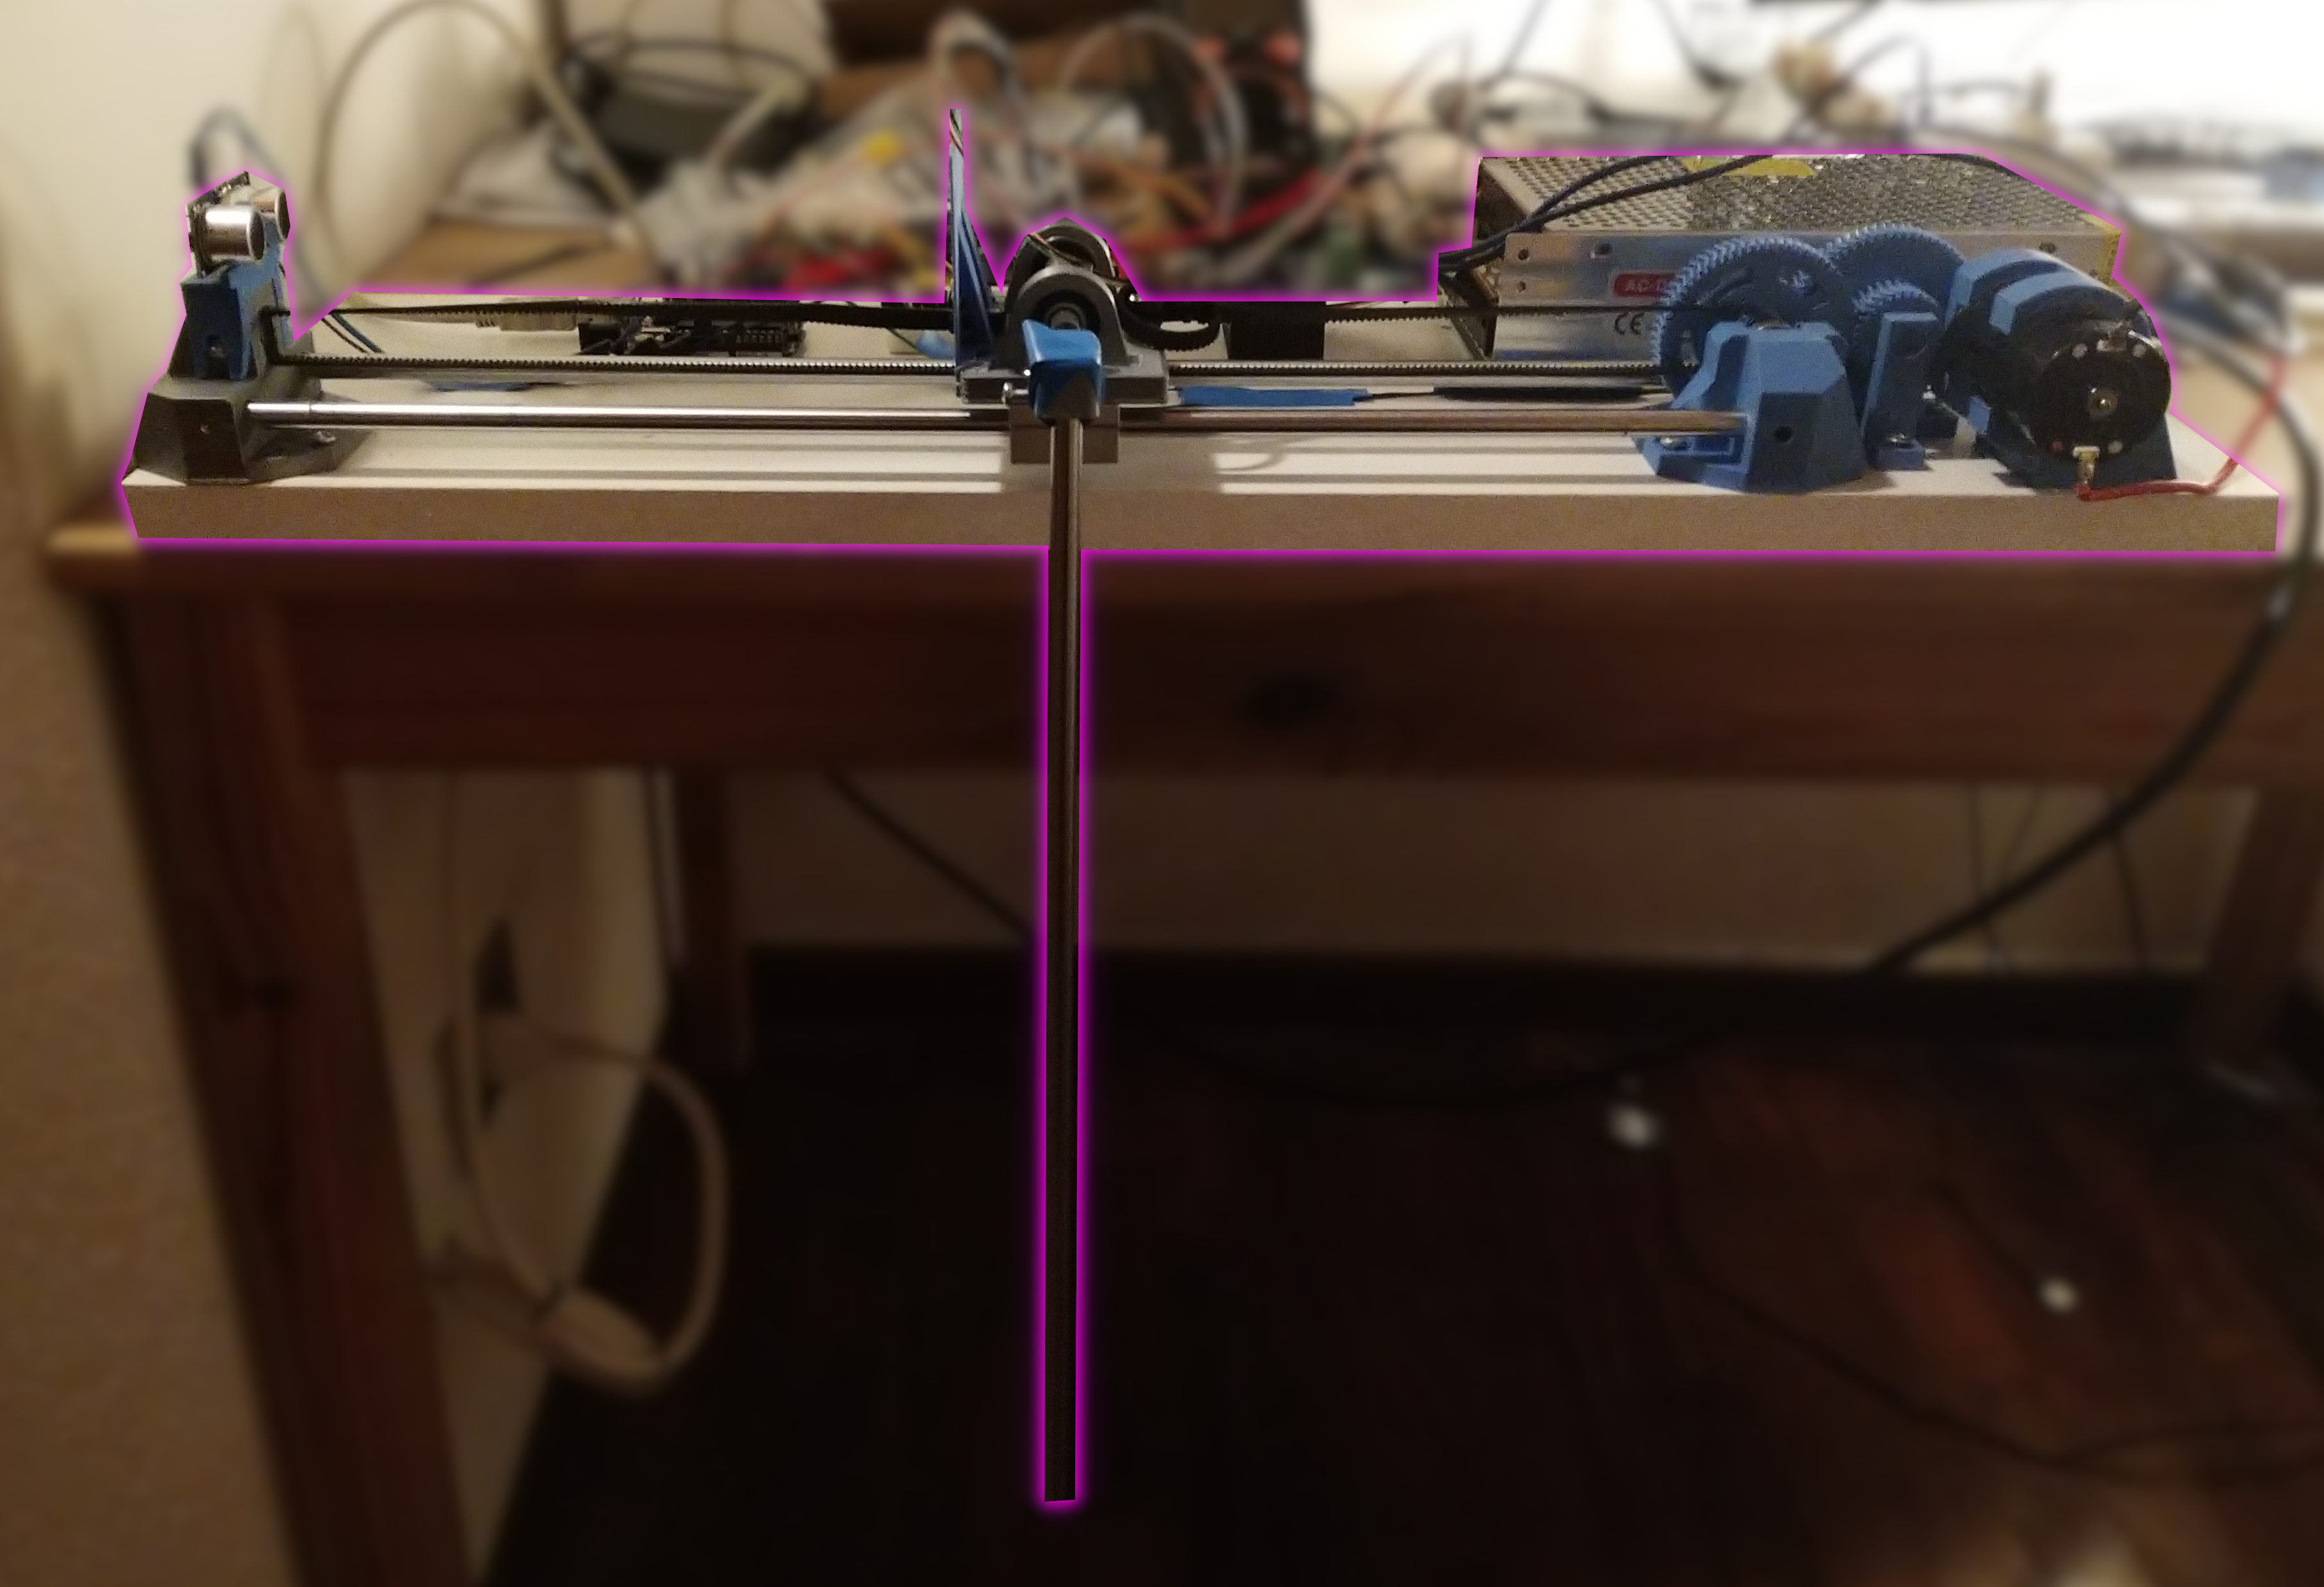
\includegraphics[width=0.47\textwidth]{../assets/pend-down.jpg}
  \caption{\emph{Pendolo invertito. Il carrello può scorrere su due rotaie a basso coefficiente d'attrito. Il motore
  controlla il carrello grazie ad una cinghia. Il pendolo è libero di ruotare, grazie a due cuscinetti.}}
  \label{fig:foto}
\end{figure}

  \section{Sviluppo del controller \textsc{LQG}}\label{sec:lqg}
\subsection{Discretizzazione del sistema}\label{subsec:discretizzazione}
Nella sezione \ref{subsec:intro-lqr} ho spiegato come funziona un controller \textsc{lqr} per sistemi a \emph{tempo continuo}.
Il sistema che ho realizzato, tuttavia, non può raccogliere dati dai sensori in modo continuo: tra un osservazione
$\mathbf y_k$ e la successiva $\mathbf y_{k+1}$ passa un certo intervallo di tempo $\Delta t$.
Tutte le considerazioni fatte finora continuano a valere, ma dal punto di vista pratico è necessario discretizzare il sistema.
Vogliamo trovare le matrici $A_d$ e $B_d$ tali cui le equazioni
\begin{equation}
  \begin{aligned}
    \mathbf{x}_{k+1} = A_d \mathbf{x}_k + B_d f_k
  \end{aligned}
  \label{eq:moto-discreto}
\end{equation}
approssimino meglio le \eqref{eq:state-space} fissato un $\Delta t > 0$.
Si può dimostrare\cite{brunton2019data}
che valgono:
\begin{equation}
  \begin{aligned}
    A_d &= e^{A\Delta t} \\
    B_d &= B\left( \int_0^{\Delta t} e^{A \tau} d\tau \right)
  \end{aligned}
  \label{eq:discrete-mapping}
\end{equation}
Tuttavia, operativamente, per $\Delta t \ll 1$, possiamo trovare velocemente una soluzione approssimata per \eqref{eq:discrete-mapping}:
\begin{equation}
  \begin{aligned}
    \mathbf x_{k+1} &\approx x_k + \dot x|_k \Delta t\\
      &\approx \mathbf x_k + (A \mathbf x_k + B f_k) \Delta t\\
      &\approx (I + \Delta t A) \mathbf x_k + B \Delta t f_k\\
  \end{aligned}
  \label{eq:discrete-mapping-approx}
\end{equation}
Le matrici che cerchiamo sono quindi:
\begin{equation}
  \begin{aligned}
  A_d &=
  \left(\begin{array}{cccc}1&\Delta t&0&0\\0&1&-\frac{3gm}{m+4M}\Delta t&0\\0&0&1&\Delta t\\0&0&-\frac{6g(m+M)}{l(m+4M)} \Delta t&1\\\end{array}\right)
  \\
  B_d &=
  \left(\begin{array}{c}0\\\frac{4}{m+4M} \Delta t\\0\\\frac{6}{lm+4lM} \Delta t\\\end{array}\right)
  \label{eq:Ad-e-Bd}
  \end{aligned}
\end{equation}

\subsection{Controllabilità del sistema}\label{subsec:controllabilità}
Prima di procedere con il calcolo dei coefficienti del controller, dobbiamo accertarci che il sistema sia \emph{controllabile}.
Condizione necessaria e sufficiente per la controllabilità è che la \emph{matrice di controllabilità}, definita in \eqref{eq:matrice-controllabilità}
abbia rango massimo\footnote{
  In realtà, è necessario anche che gli autovalori di $A$ non abbiano la forma $\frac {2k\pi i} {\Delta t}, \forall k \in \mathbb Z_0$.
  Si può verificare facilmente questa condizione fissando qualche valore numerico (cosa che farò nella sezione \ref{sec:risultati}); per
  ora assumerò che sia soddisfatta (in ogni caso, gli autovalori di $A$ dipendono solo da parametri razionali, quindi è
  pressochè impossibile che assumano valori multipli di $\pi$).
}%
\footnote{
  Questo test per la controllabilità non mi da alcuna informazione su \emph{quanto} sia controllabile il mio sistema.
  Esistono altri metodi che permettono di ottenere queste informazioni (e.g. si può calcolare il Gramiano
  $W=\int_0^{+\infty}e^{As}BB^*e^{A^*s}\ ds$ e studiarne gli autovalori).
}
\cite{sontag2013mathematical}.

\begin{framed}
  \textbf{DEF} Matrice di controllabilità
  \begin{equation}
    \mathcal C_d \doteq \left[
      \begin{matrix}
        B_d & A_dB_d & A_d^2B_d & \ldots & A_d^{n-1}B_d
      \end{matrix}
      \right]
    \label{eq:matrice-controllabilità}
  \end{equation}
\end{framed}

Svolgendo i calcoli, si trova che il sistema \eqref{eq:A-e-B} è sempre controllabile\footnote{Assumendo che tutti i
parametri siano positivi.}.

\subsection{Calcolo dei coefficienti del controller}\label{calcolo-coefficienti}
Definisco la funzione costo per il sistema \eqref{eq:discrete-mapping}:
\begin{equation}
  J(t) =
  \sum_{k=0}^{+\infty} \left[ \mathbf{x}_k^* Q \mathbf {x}_k + f_k R f_k \right]
  \label{eq:lqr-costo-discreto}
\end{equation}
si può dimostrare\cite{chow1975analysis} che la soluzione $f = f(\mathbf x)$ ottimale per il problema di controllo al tempo $t = k \Delta t$ è data da:
% yeet subscript t per infinite horizon problem
\begin{equation}
  \begin{aligned}
  f_k^{\text{opt}}(\mathbf x) &= -K y_{k-1} \\
  \text{con}\ K &= (B_d^*PB_d + R)^{-1}(B_d^*PA_d)
  \end{aligned}
  \label{eq:f-opt}
\end{equation}
dove $P$ è la soluzione all'equazione di Ricciati a tempo discreto (\textsc{dare})\eqref{eq:ricciati}:%
\begin{framed}
  \textbf{DEF} \textsc{dare}
  \begin{equation}
    \begin{aligned}
    P &=A_d^* P A_d\ - \\
     &-(A_d^* P B_d)(R + B_d^* P B_d)^{-1}(B_d^* P A_d)\ + \\
    &+ Q
    \end{aligned}
    \label{eq:ricciati}
  \end{equation}%
\end{framed}%
Calcolare i coefficienti del controller significa risolvere l'equazione \eqref{eq:ricciati} e trovare il vettore $K$.

%todo spiega come mai c'è da risolvere equazione di ricciati

  \section{Sviluppo del controller \textsc{PID}}\label{sec:pid}
Non ci sono molte considerazioni da fare riguardo allo sviluppo di questo controller.
Si procede alla ricerca dei coefficienti con il metodo \emph{trial-and-error}, controllando prima l'angolo $\theta$ e
poi la posizione $x$.
Ho scelto di non includere il termine integrale nel controller, visto che per questa applicazione non è necessario.
L'espressione finale per $u$ è:

\begin{equation}
  \begin{aligned}
  u(t) &= K_{p\theta}\theta + K_{d\theta}\frac{d(\theta - \theta_0)}{dt} +\\
  &+ K_{px}x + K_{dx}\frac{d(x - x_0)}{dt}
  \end{aligned}
  \label{eq:pid-control}
\end{equation}


  \section{Risultati}\label{sec:risultati}
I valori numerici dei coefficienti per i controller \textsc{lqr} e \textsc{pid} sono riportati in appendice \ref{sec:parametri-sistema}
rispettivamente in tabella \ref{tab:coefficienti-lqr} e \ref{tab:coefficienti-pid}.
Usando questi parametri, il pendolo rimane rovesciato (figura )%todo add foto
Tutto il codice usato per stabilizzare il pendolo e calcolare i parametri è disponibile sul mio GitHub\cite{github}.

Per avere un'idea concreta dei risultati, ho integrato il sistema usando entrambi i controller\footnote{Raccogliere
i dati del sistema fisico vero è possibile ma poco pratico. Integrando a computer ho dei grafici più chiari e, soprattutto,
confrontabili tra di loro (i.e. hanno le stesse condizioni iniziali).} (figure \ref{fig:int-lqr} e \ref{fig:int-pid}).
Il risultato è compatibile con quello che si osserva per il sistema reale.
Ho integrato anche $f^*f$ per entrambi i sistemi; il risultato è:
\begin{equation}
  \frac {E_{LQR} } {E_{PID}} \approx \frac 3 5
  \label{eq:rapporto-f}
\end{equation}

Aggiungo anche che, qualitativamente, ho osservato che il controller \textsc{lqr} funziona meglio del \textsc{pid}, ma
richiede che i dati in input dei sensori siano più \emph{puliti}.

\begin{figure}[h]
  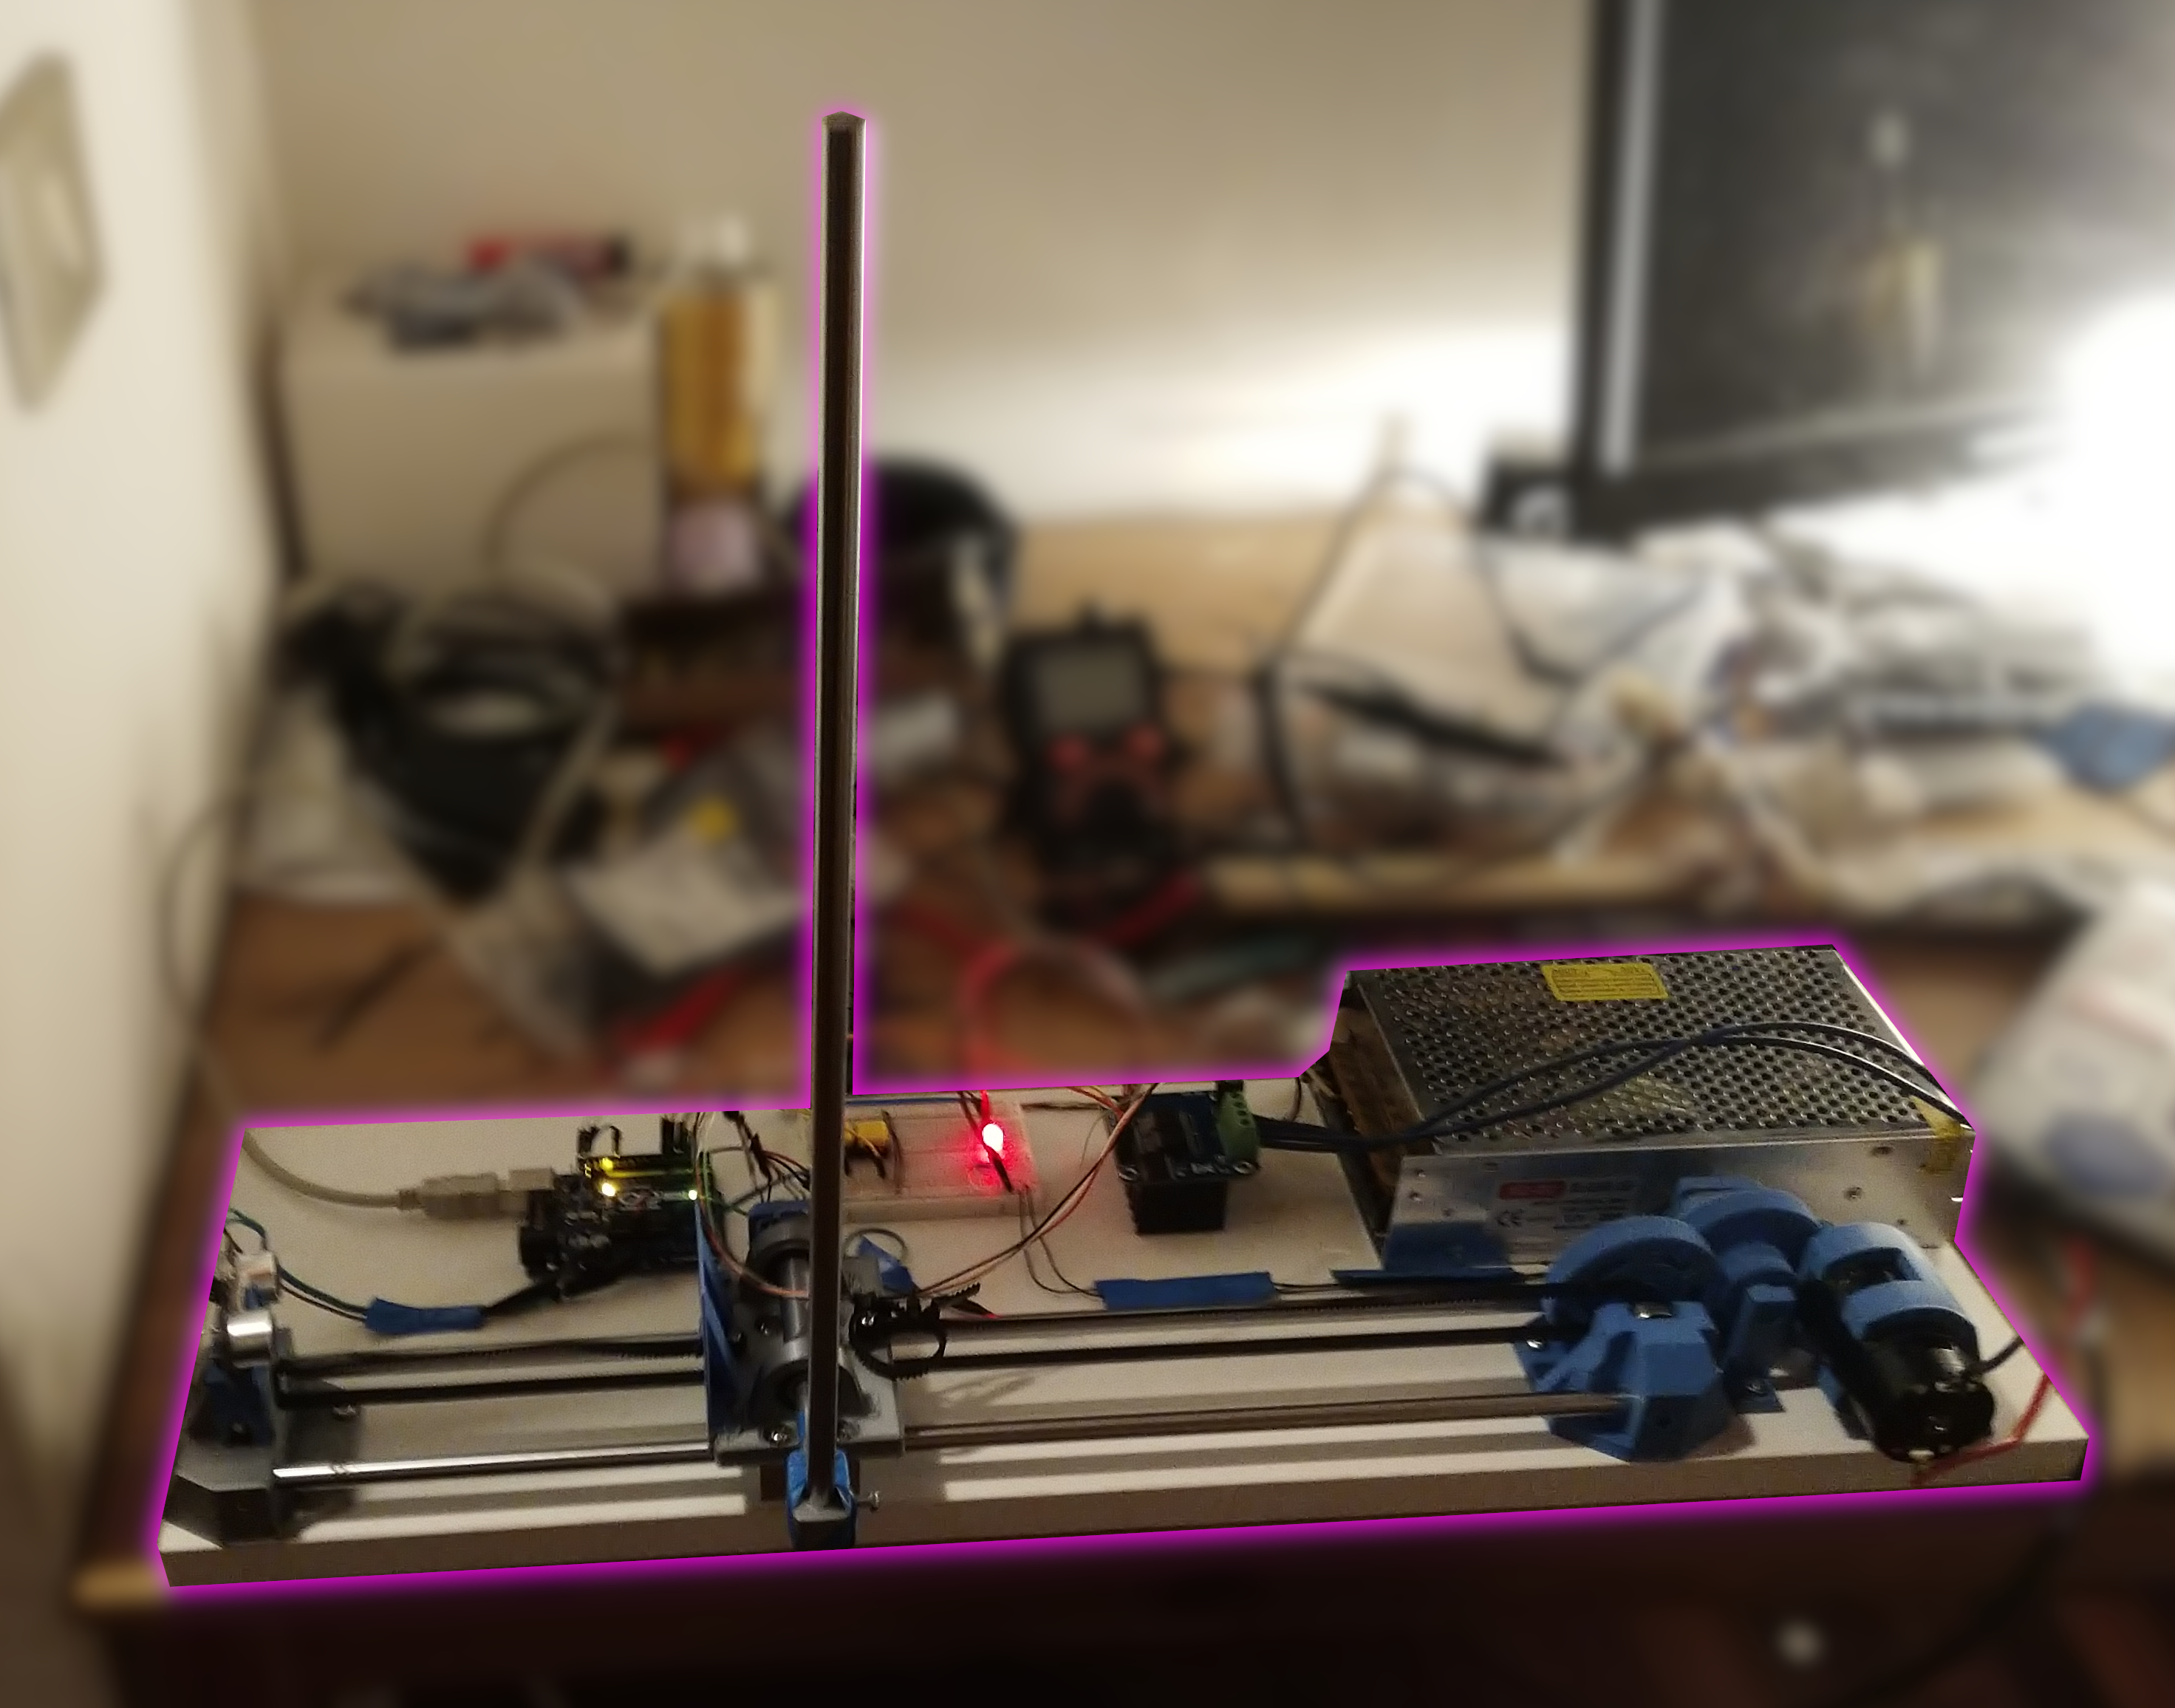
\includegraphics[width=0.5\textwidth]{pend-up.jpg}
  \caption{\emph{Sistema del pendolo invertito stabilizzato.}}
  \label{fig:pend-up}
\end{figure}

\begin{figure}[h]
  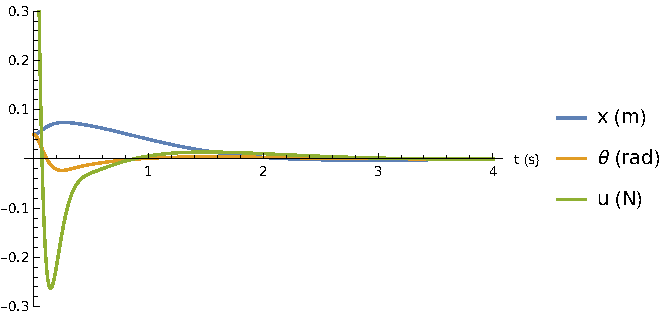
\includegraphics[width=0.47\textwidth]{integrazione lqr.pdf}
  \caption{\emph{Sistema controllato con LQR; il controller lineare è applicato alle equazioni vere del moto.}}
  \label{fig:int-lqr}
\end{figure}

\begin{figure}[h]
  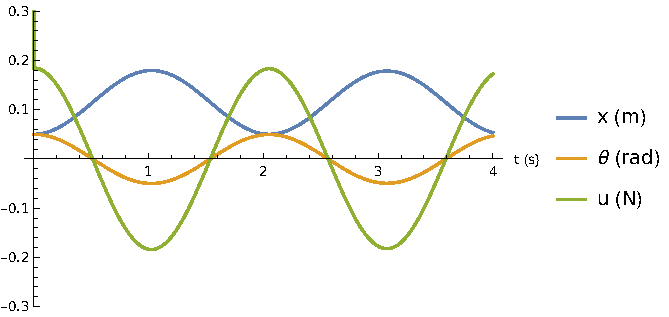
\includegraphics[width=0.47\textwidth]{integrazione pid.pdf}
  \caption{\emph{Sistema controllato con PID; il controller è applicato alle equazioni vere del moto.}}
  \label{fig:int-pid}
\end{figure}




  \section{Conclusioni}\label{sec:conclusioni}

  \section{Approfondimenti}\label{sec:approfondimenti}
6

  \appendix
\section{Parametri del sistema}\label{sec:parametri-sistema}
\begin{table}[H]
  \centering
  \begin{tabular}[t]{cc}
    \toprule
    Parametro &Valore\\
    \midrule
    $m$ & $.150$Kg \\
    $M$ & $.175$Kg \\
    $L$ & $.38$m   \\
    $g$ & $9.8\frac {\text m}{\text {s}^2}$ \\
    \bottomrule
  \end{tabular}
  \caption{
    Parametri del sistema.
  }
  \label{tab:parametri-sistema}
\end{table}

\begin{table}[H]
  \centering
  \begin{tabular}[t]{cc}
    \toprule
    Parametro &Valore\\
    \midrule
    \vspace{5px}
    $Q$ & $\left(\begin{matrix}
                   &.1 &0 &0 &0 \\ &0 &.0001 &0 &0 \\ &0 &0 &1 &0 \\ &0 &0 &0 &.0001
    \end{matrix}\right)$ \\
    \vspace{5px}
    $R$ & $\left(\begin{matrix}
                   .005
    \end{matrix}\right)$ \\
    \vspace{5px}
    $K$ & $\left(\begin{matrix}
                   3.67 \\ 3.85 \\ 22.6 \\ 3.97
    \end{matrix}\right)$ \\
    $\Delta t$ & $20$ms \\
    \bottomrule
  \end{tabular}
  \caption{
    Parametri adimensionali del controller \textsc{lqr}. Le matrici $Q$ e $R$ sono definite da me, $K$ è stato ricavato.
  }
  \label{tab:coefficienti-lqr}
\end{table}

\begin{table}[H]
  \centering
  \begin{tabular}[t]{cc}
    \toprule
    Parametro &Valore\\
    \midrule
    $K_{px}$ & $2$ \\
    $K_{dx}$ & $1000$ \\
    $K_{p\theta} $ & $15$   \\
    $K_{d\theta}$ & $1300$ \\
    \bottomrule
  \end{tabular}
  \caption{
    Parametri adimensionali del controller \textsc{pid}, ricavati con il metodo \emph{trial-and-error}.
  }
  \label{tab:coefficienti-pid}
\end{table}

\section{Calibrazione del motore}\label{sec:calibrazione-motore}
Un motore DC è controllato variando il voltaggio $V$ in ingresso. La forza esercitata dal motore, tuttavia, non è
lineare rispetto a $V$. Per risolvere questo problema, possiamo usare la formula\cite{dcControl}:
  \begin{equation}
    \begin{aligned}[c]
      u_k = \frac {(1-a)v_k -c \text{sign} v_k + \Delta t \dot v_k} {b}
    \end{aligned}
    \label{eq:motore}
  \end{equation}

Ho ricavato i parametri $a$, $b$ e $c$ dal fit in figura \ref{fig:fit}; i valori numerici sono riportati in tabella \ref{tab:fit}.

\begin{figure}[h]
  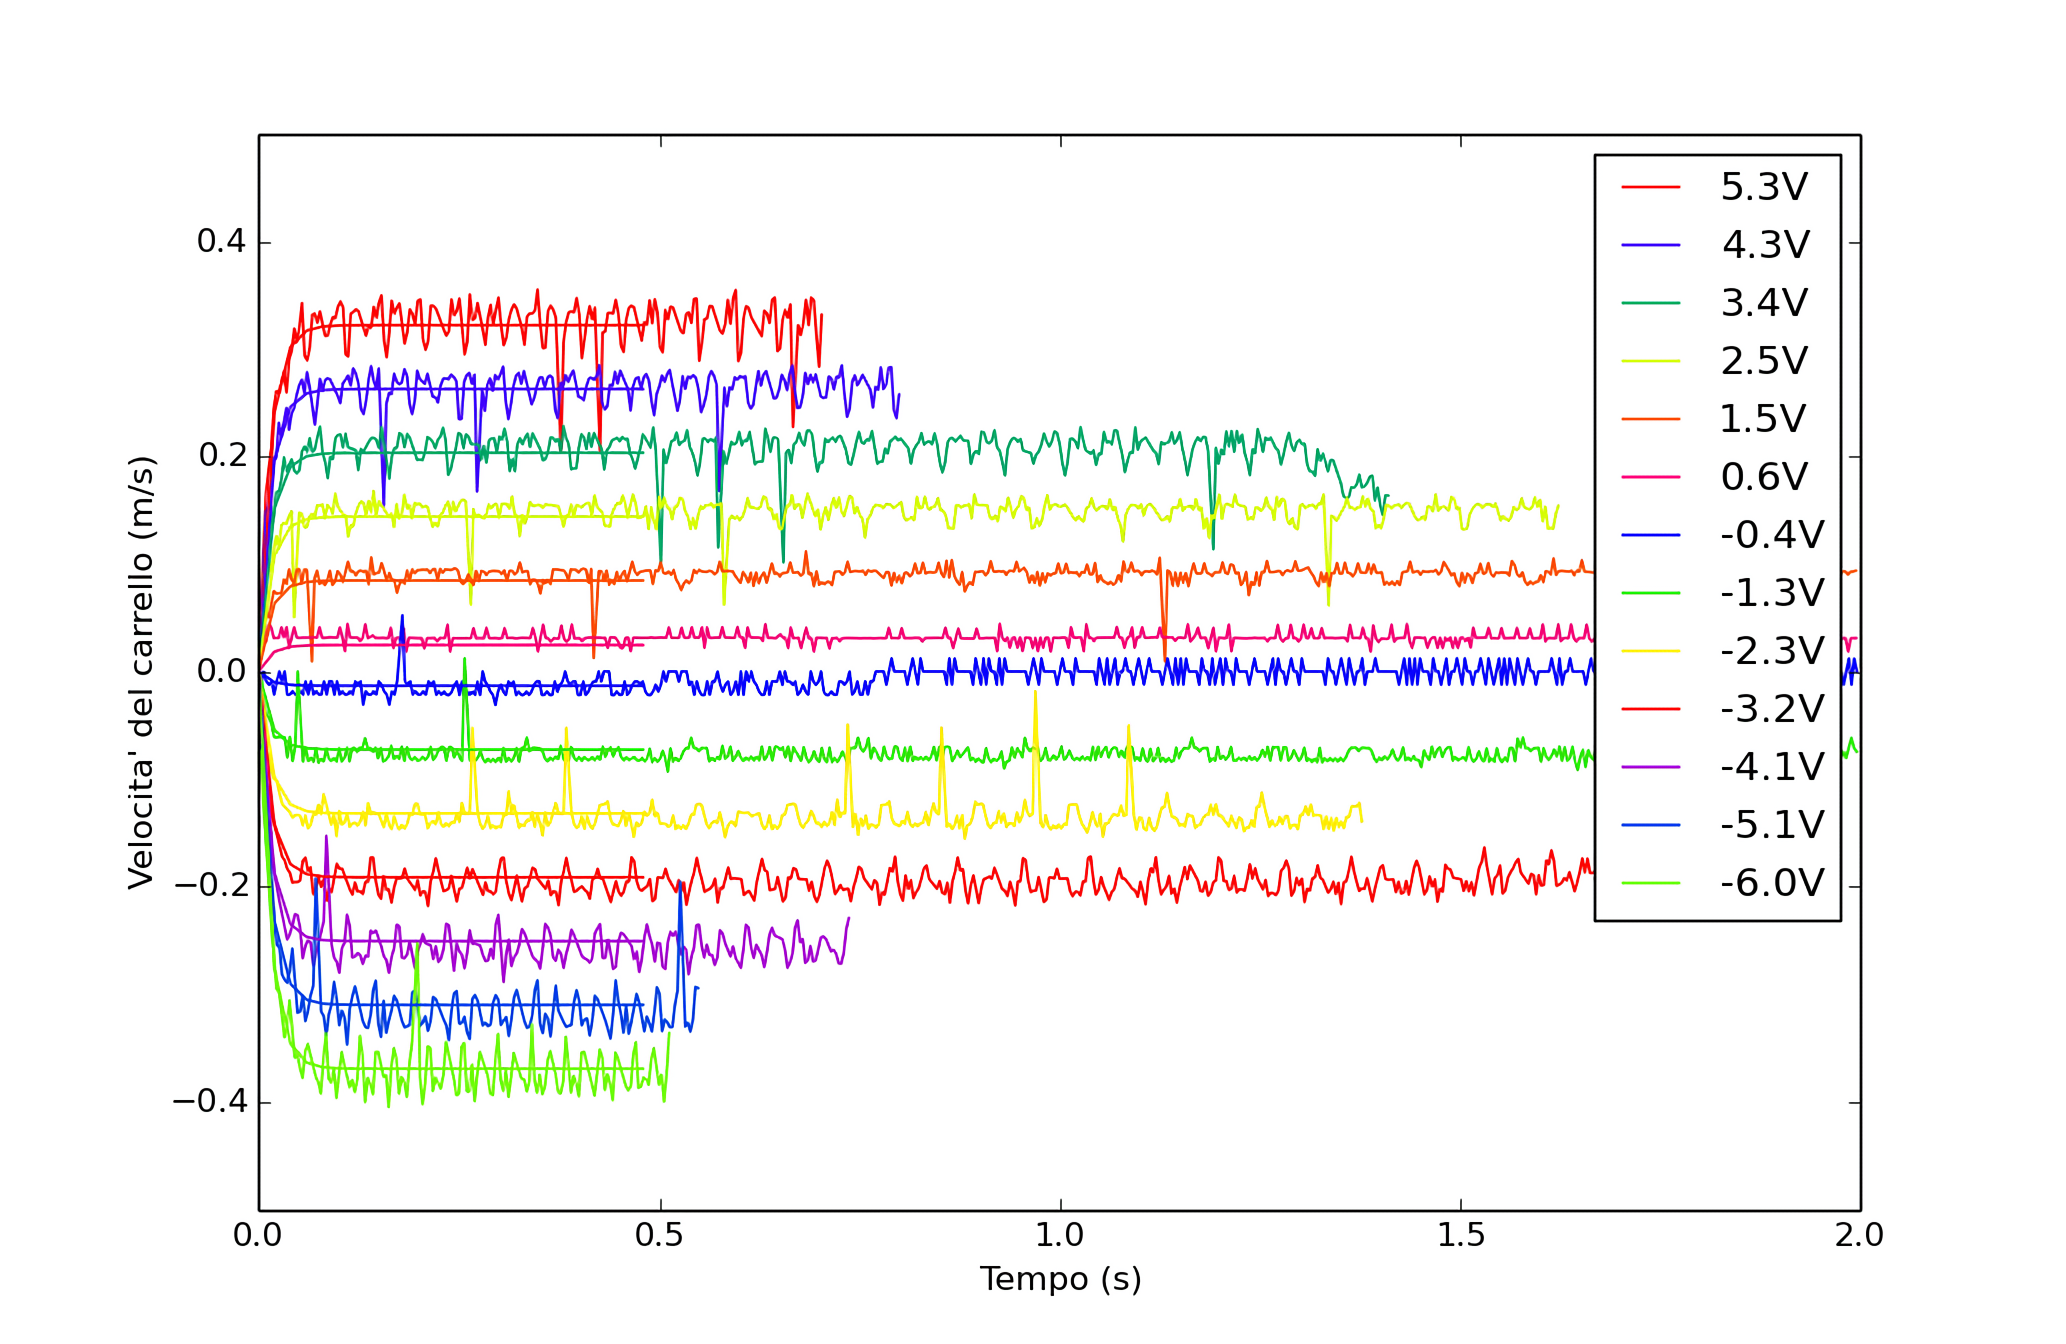
\includegraphics[width=0.47\textwidth]{../assets/fit.png} %todo cambia
  \caption{\emph{Fit dei parametri del motore.}}
  \label{fig:fit}
\end{figure}

\begin{table}[H]
  \centering
  \begin{tabular}[t]{cc}
    \toprule
    Parametro &Valore\\
    \midrule
    $a$ & $.251$ \\
    $b$ & $.047$ \\
    $c$ & $.008$ \\
    \bottomrule
  \end{tabular}
  \caption{
    Parametri adimensionali ottenuti dal fit del motore.
  }
  \label{tab:fit}
\end{table}





\bibliographystyle{unsrt} % We choose the "plain" reference style
\bibliography{invertedPendulumRefs}
\end{document}
